% This is the main file for the template for doctoral thesis at
% University of Zagreb, Faculty of Electrical Engineering and Computing
% in Zagreb, Croatia.
% Initial version was created in April 2013, last update was in July 2014.

% Author: Jelena Bozek, jelena.bozek@fer.hr
% Contributor: Vedran Miletic, vmiletic@inf.uniri.hr


%%%%%%%%%%%%%%%%%%%%%%%%% POSTAVKE / SETTINGS %%%%%%%%%%%%%%%%%%%%%%%%%%%%%
\documentclass[12pt,oneside, a4paper]{book}
\usepackage{etex}
\usepackage{xcolor}
\usepackage[pdftex]{graphicx}
\usepackage{rotating}
\usepackage{epsfig}
\usepackage{epstopdf}
% required for printing index
% use \index{name} in text
%\usepackage{makeidx}
%\makeindex
% required for printing nomenclature
% use \nomenclature{symbol}{description} in text
%\usepackage{nomencl}
%\makenomenclature
%\renewcommand{\nomname}{Popis oznaka}

\usepackage[T1]{fontenc}
\usepackage[utf8]{inputenc}
\usepackage{cmap}
\usepackage[english]{babel}
\usepackage{ae}
\usepackage[unicode]{hyperref}
\usepackage{mathptmx}
\usepackage{amscd}
\usepackage{amssymb}
\usepackage{amsmath}
\usepackage{amsfonts}

\usepackage[left=2.5cm,right=2.5cm,top=2.5cm,bottom=2.5cm]{geometry}
\usepackage{setspace} 
\linespread{1.3}
\usepackage{fancyhdr} % setting up header and position of page numbers
\pagestyle{fancyplain}
\fancyhf{}
\lhead{\nouppercase{\fancyplain{}{\leftmark}}}
\renewcommand{\chaptermark}[1]{\markboth{#1}{}}
\rfoot{\thepage}

\usepackage{hhline}
\usepackage{enumerate}
\usepackage{delarray}
\usepackage{array}  % package for some table properties
\usepackage{tabularx} % package that allows dynamical changing table cell width
\usepackage{multirow}  % package that enables multiple rows in a table
\usepackage[bf, font=small]{caption}
\usepackage[labelfont=small, font=small]{subcaption}
\usepackage{wasysym}
\usepackage{subeqnarray}
\usepackage{aeguill}
\usepackage{pdflscape} % setting page into landscape view
\usepackage{enumitem} % for itemize lists
\setlist{nolistsep}   % setting for itemize lists

\renewcommand{\thefootnote}{\fnsymbol{footnote}}  % to get unnumbered footnotes
\renewcommand{\arraystretch}{1.5} % stretching row height

\usepackage[square, numbers, sort]{natbib} 
% change the name of Bibliography heading into "Literatura"
% \addto\captionscroatian{%
%   \renewcommand{\bibname}{Bibliography}
% }

% Adding a dot after chapter number in TOC 
\let\savenumberline\numberline
\def\numberline#1{\savenumberline{#1.}}

% Adding dots after chapter titles to page number in TOC
\makeatletter
\renewcommand*\l@chapter[2]{%
  \ifnum \c@tocdepth >\m@ne
  \addpenalty{-\@highpenalty}%
  \vskip 1.0em \@plus\p@
  \setlength\@tempdima{1.5em}%
  \begingroup
  \parindent \z@ \rightskip \@pnumwidth
  \parfillskip -\@pnumwidth
  \leavevmode \bfseries
  \advance\leftskip\@tempdima
  \hskip -\leftskip
  #1\nobreak\normalfont\leaders\hbox{$\m@th
    \mkern \@dotsep mu\hbox{.}\mkern \@dotsep
    mu$}\hfill\nobreak\hb@xt@\@pnumwidth{\hss #2}\par
  \penalty\@highpenalty
  \endgroup
  \fi}
\makeatother

% adjust the line spacing in a matrix
\makeatletter
\renewcommand*\env@matrix[1][\arraystretch]{%
  \edef\arraystretch{#1}%
  \hskip -\arraycolsep
  \let\@ifnextchar\new@ifnextchar
  \array{*\c@MaxMatrixCols c}}
\makeatother

% remove footer (page number) from TOC, list of figures and list of tables
\AtBeginDocument{\addtocontents{toc}{\protect\thispagestyle{empty}}}
\AtBeginDocument{\addtocontents{lof}{\protect\thispagestyle{empty}}}
\AtBeginDocument{\addtocontents{lot}{\protect\thispagestyle{empty}}}


\begin{document}


%%%%%%%%%%%%%%%%%%%%%%%%%%%%%%%%%%%%%%%%%%%%%%%%%%%%%%%%%%%%%%%%%%%%%%%%%%%
\frontmatter

%%%%%%%%%%%%%%%%%%%% NASLOVNICA / FRONT COVER PAGE %%%%%%%%%%%%%%%%%%%%%%%%
\begin{titlepage}
  \fontsize{16pt}{20pt}\selectfont
  \fontfamily{phv}\fontseries{mc}\selectfont
  \newgeometry{left=3cm,right=3cm,top=3cm,bottom=2.5cm}
  \setlength{\intextsep}{0pt plus 0pt minus 0pt}

  \begin{center}
    \begin{figure}[ht!]
      \begin{center}
        
\includegraphics[height=4.1184cm, width=5.94cm]{logo_unizg_eng}
      \end{center}
    \end{figure}
    \vspace{0cm}
    {FACULTY OF ELECTRICAL ENGINEERING AND COMPUTING} \\
    \vspace{3cm}
    Filip Boltužić \\
    \vspace{2cm}
    {\fontsize{22pt}{22pt}\selectfont
\textbf{
COMPUTATIONAL METHODS FOR ARGUMENTATION MINING OF CLAIMS IN INTERNET DISCUSSIONS}} \\
    \vspace{2cm}  
    DOCTORAL THESIS \\    
    \vfill{Zagreb, 2019}
  \end{center}
  \restoregeometry
\end{titlepage}

%%%%%%%%%%%%%% DRUGA UNUTARNJA STRANICA / SECOND INNER PAGE %%%%%%%%%%%%%%%
\begin{titlepage}
  \fontsize{16pt}{20pt}\selectfont
  \fontfamily{phv}\fontseries{mc}\selectfont
  \newgeometry{left=3cm,right=3cm,top=3cm,bottom=2.5cm}
  \setlength{\intextsep}{0pt plus 0pt minus 0pt}

  \begin{center}
    \begin{figure}[ht!]
      \begin{center}
        
\includegraphics[height=4.1184cm, width=5.94cm]{logo_unizg_eng}
      \end{center}
    \end{figure}		
    \vspace{0cm}
    {\fontsize{16pt}{16pt}{FACULTY OF ELECTRICAL ENGINEERING AND COMPUTING}} \\
    \vspace{3cm}
    Filip Boltužić \\
    \vspace{2cm}
    {\fontsize{22pt}{22pt}\selectfont\textbf{
COMPUTATIONAL METHODS FOR ARGUMENTATION MINING OF CLAIMS IN INTERNET DISCUSSIONS}} \\
    \vspace{2cm}   
    DOCTORAL THESIS \\  
    \vspace{5cm}   % adjust this spacing if necessary
    Supervisor: Associate Professor Jan Šnajder, PhD \\
    \vfill{Zagreb, 2019}
  \end{center}
  \restoregeometry
\end{titlepage}

%%%%%%%%%%%%%%% PRVA UNUTARNJA STRANICA / FIRST INNER PAGE %%%%%%%%%%%%%%%%
\begin{titlepage}
  \fontsize{16pt}{20pt}\selectfont
  \fontfamily{phv}\fontseries{mc}\selectfont
  \newgeometry{left=3cm,right=3cm,top=3cm,bottom=2.5cm}
  \setlength{\intextsep}{0pt plus 0pt minus 0pt}

  \begin{center}
    \begin{figure}[ht!]
      \begin{center}
        
\includegraphics[height=4.1184cm, width=5.94cm]{logo_unizg2}
      \end{center}
    \end{figure}		
    \vspace{0cm}
    {FAKULTET ELEKTROTEHNIKE I RAČUNARSTVA} \\
    \vspace{3cm}
    Filip Boltužić \\
    \vspace{2cm}
    {\fontsize{22pt}{22pt}\selectfont\textbf{
RAČUNALNI POSTUPCI DUBINSKE ARGUMENTATIVNE ANALIZE TVRDNJI U INTERNETSKIM RASPRAVAMA
}} \\
    \vspace{2cm}    
    DOKTORSKI RAD \\
    \vspace{5cm}    % adjust this spacing if necessary
	Mentor: Izv. Prof. dr. sc. Jan Šnajder \\
    \vfill{Zagreb, 2019.}
  \end{center}
  \restoregeometry
\end{titlepage}


%%%%%%%%%%%%%%%%%%%%%%%%%%%%%%%%%%%%%%%%%%%%%%%%%%%%%%%%%%%%%%%%%%%%%%%%%%%
\begin{titlepage}
  \begin{minipage}{\dimexpr\textwidth-1cm}
    \vspace{3cm}
    Doktorski rad izrađen je na Sveučilištu u Zagrebu
    Fakultetu elektrotehnike i računarstva, na Zavodu za 
    elektroniku, mikroelektroniku, računalne i inteligentne sustave, u 
    Laboratoriju za analizu teksta i inženjerstvo znanja (TakeLab).

    \vspace{1cm}
    Mentor: izv. prof. dr. sc. Jan Šnajder

    \vspace{1cm}
    Doktorski rad ima: XYZ stranica

    \vspace{1cm}
    Doktorski rad br.: \line(1,0){64}
  \end{minipage}
\end{titlepage}

%%%%%%%%%%%%%%%%%%%%%%%%%%%%%%%%%%%%%%%%%%%%%%%%%%%%%%%%%%%%%%%%%%%%%%%%%%%
% insert info page about supervisor which is saved in separate file
\thispagestyle{empty}

\section*{About the Supervisor}


Short biography of the supervisor.


\section*{O mentoru}


Kratki životopis mentora.


%%%%%%%%%%%%%%%%%%%%%%%%%%%%%%%%%%%%%%%%%%%%%%%%%%%%%%%%%%%%%%%%%%%%%%%%%%%
% insert optional page with thanks or dedication
%\include{eg_thanks_dedication}

%%%%%%%%%%%%%%%%%%%%%%%%%%%%%%%%%%%%%%%%%%%%%%%%%%%%%%%%%%%%%%%%%%%%%%%%%%%
% insert page with abstract
\thispagestyle{empty}


\section*{Sažetak}

Ovo je \LaTeX\ predložak za doktorski rad izrađen na Sveučilištu u Zagrebu
Fakultetu elektrotehnike i računarstva. Osnovna datoteka  koja služi za
izgradnju konačne PDF dadoteke je main.tex. U datoteci main.tex oblikovane su
uvodne stranice rada, a naredbom \textit{include} umeću se dodatne stranice i
dodaju poglavlja. U predlošku su umetnute datoteke eg\_supervisor.tex
(predložak za biografiju mentora na hrvatskom i engleskom jeziku),
eg\_thanks\_dedication.tex (predložak za opcionalnu stranicu sa zahvalama i/ili
posvetom), eg\_abstract.tex (predložak za sažetak), (predložak za sažetak)
eg\_prosireni\_sazetak.tex (predložak za prošireni sažetak na hrvatskom
jeziku), eg\_extended\_abstract.tex (predložak za prošireni sažetak na
engleskom jeziku), eg\_chapter.tex (primjer jednog poglavlja rada),
eg\_zivotopis.tex (predložak za životopis autora na hrvatskom jeziku) te
eg\_biography.tex (predložak za životopis na engleskom jeziku).

\vspace{1cm}
\textbf{Ključne riječi}:  doktorski rad, \LaTeX, FER


\section*{Abstract}


Abstract.

\vspace{1cm}
\textbf{Keywords}:  doktorski rad, \LaTeX, FER


%%%%%%%%%%%%%%%%%%%%%%%%%%%%%%%%%%%%%%%%%%%%%%%%%%%%%%%%%%%%%%%%%%%%%%%%%%%
% insert page with extended abstract
% prošireni sažetak na hrvatskom, ako rad nije pisan na tom jeziku
%\include{eg_prosireni_sazetak}
% prošireni sažetak na engleskom, ako rad nije pisan na tom jeziku
\include{eg_extended_abstract}

%%%%%%%%%%%%%%%%%%%%%%%%%%%%%%%%%%%%%%%%%%%%%%%%%%%%%%%%%%%%%%%%%%%%%%%%%%%
\clearpage
%%%%%%%%%%%%%%%%%%%%%%%%%%%%%%%%% TOC %%%%%%%%%%%%%%%%%%%%%%%%%%%%%%%%%%%%%
\pagestyle{empty} % remove header/footer 
\tableofcontents
\cleardoublepage % start new page

\pagestyle{fancyplain} % puts headers/footers back on


%%%%%%%%%%%%%%%%%%%%%%%%%%%%%%%%%%%%%%%%%%%%%%%%%%%%%%%%%%%%%%%%%%%%%%%%%%%
\mainmatter
%%%%%%%%%%%%%%%%%%%%%%%% POGLAVLJA / CHAPTERS %%%%%%%%%%%%%%%%%%%%%%%%%%%%%



\chapter{Uvod}

U ovom poglavlju prikazane su neke od funkcije koje se mogu koristiti prilikom
oblikovanja rada i prikaza rezultata istraživanja korištenjem \LaTeX a.

\section{Matematički izraz}


Primjer matematičke formule prikazan je izrazom

\begin{equation}
  T: \mathbf{x}_B \mapsto \mathbf{x}_A \Leftrightarrow T(\mathbf{x}_B) = \mathbf{x}_A.
  \label{eq:transformacija}
\end{equation}


\section{Slika}


Slika \ref{fig:roc_example} služi kao primjer ubacivanja slike u tekst.

\begin{figure}
  \centering
  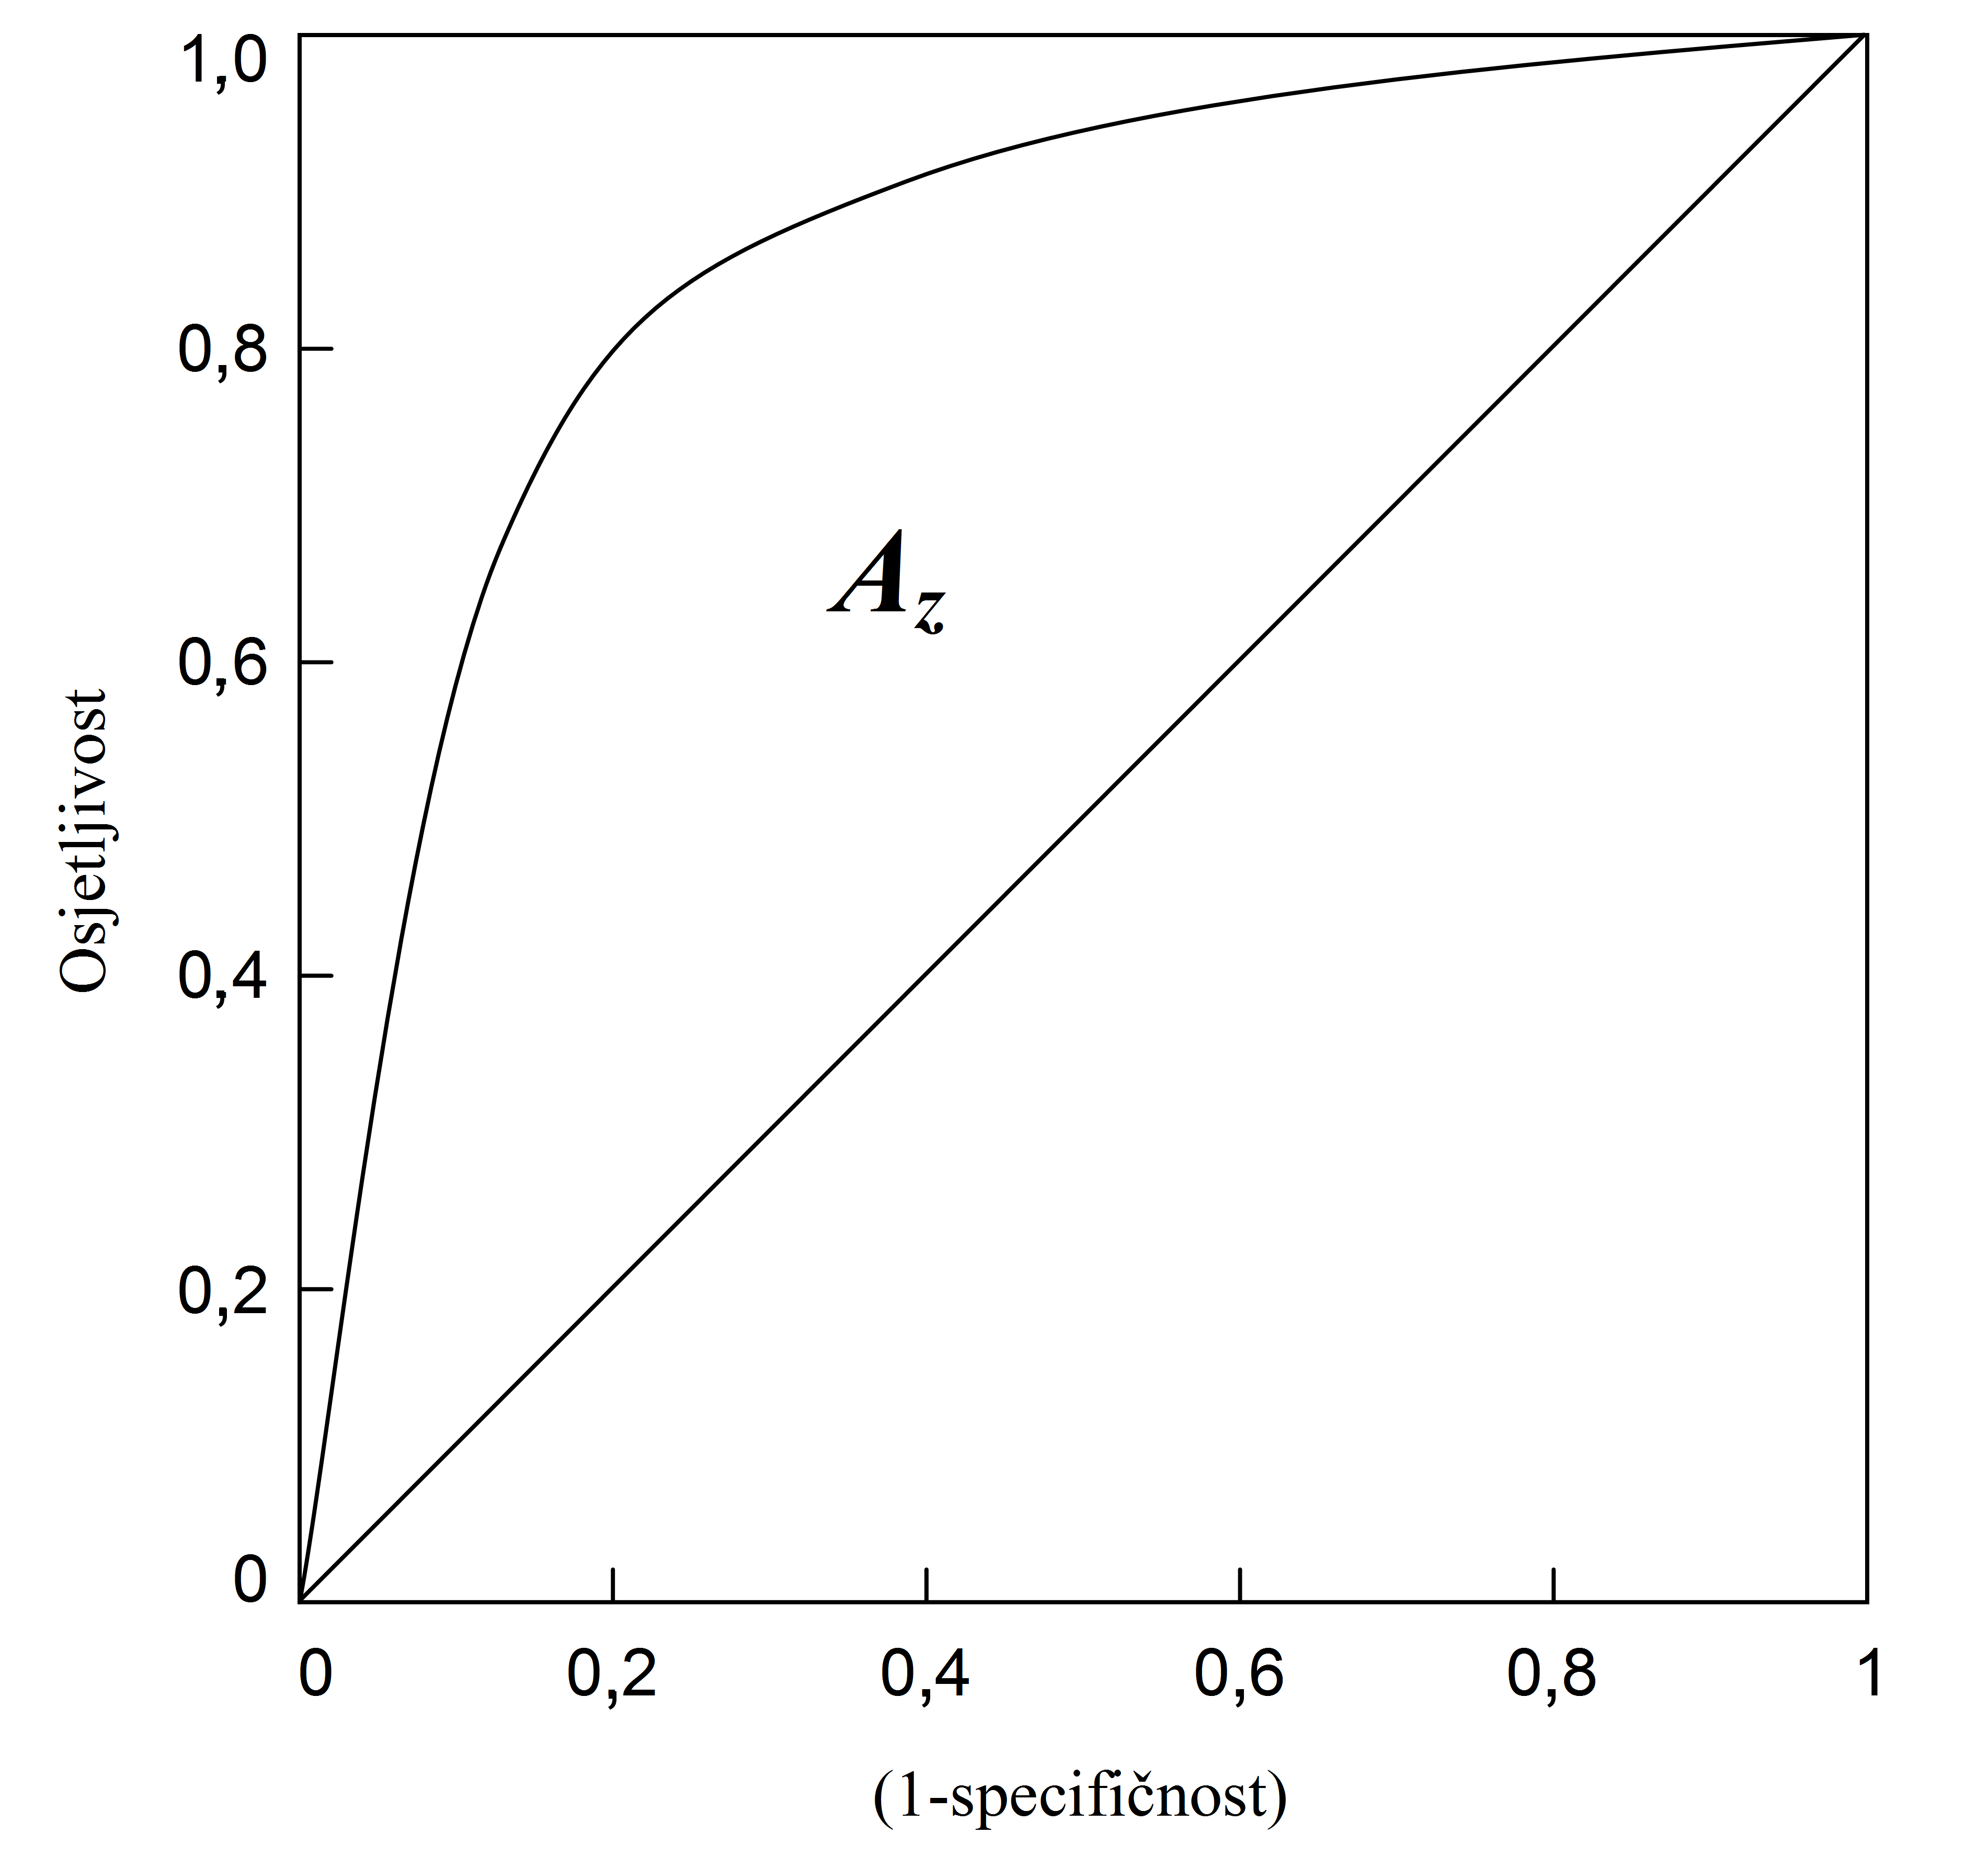
\includegraphics[width=0.7\textwidth]{roc_example}
  \caption{Primjer krivulje ROC}
  \label{fig:roc_example}
\end{figure}


\section{Tablica}


Formiranje tablice prikazano je na primjeru matrice podudarnosti u Tablici
\ref{tab:confusion_matrix}.

\begin{table} [!ht]
  \caption{Matrica podudarnosti}
  \centering  
  \begin{tabularx}{0.5\textwidth}{ c  c | c | c |}

    \cline{3-4}
    & & \multicolumn{2}{c|} {Predviđeno (\textit{predicited})}  \\ \cline{3-4}
    & & Negativno & Pozitivno \\ \cline{1-4}
    \multicolumn{1}{ |c } {\multirow{2}{*}{\rotatebox{90}{\parbox[c]{1.4cm} {Stvarno \\ (\textit{actual})}}}}  & \multicolumn{1}{ |c| }{Negativno} & NN & LPN \\ \cline{2-4}
    \multicolumn{1}{ |c  }{} & \multicolumn{1}{ |c| }{Pozitivno} & LNN & PN \\ \cline{1-4}

  \end{tabularx}
  \label{tab:confusion_matrix}
\end{table}

\subsection{\textit{Landscape}}

Postavljanja stranice u prikaz \textit{landscape} prikazano je umetanjem Tablice \ref{tab:mean_mias} u \textit{landscape}. Prikazano je i dodavanje \textit{footnotea} u tablicu.

\begin{landscape}
  \begin{table}
    % tekst u uglatim zagradama koje slijede \caption prikazuje se u Popisu tablica, a tekst u vitičastim zagradama koje slijede \caption prikazuje se iznad same tablice
    \caption[Srednje vrijednosti mjera sličnosti slika za bazu
	  mini-MIAS]{Srednje vrijednosti mjera sličnosti lijevog i desnog
	  mamograma prije i poslije registracije vođene različitim funkcijama
	  troška. Rezultati su prikazani za asimetrične (A) i normalne (N)
	  slučajeve u bazi mini-MIAS.}
    \begin{minipage}{\linewidth}   %minipage adjusts for its own footnotes
      \setcounter{mpfootnote}{\value{footnote}}
      \renewcommand{\thempfootnote}{\fnsymbol{mpfootnote}} 
      % \makebox[\textwidth] {          % center table on the page since it's wider than the page margins
      \newcolumntype{C}{>{\centering\arraybackslash}X}%
      \begin{tabularx} {\linewidth}{l C C C C C C C C C C C C} %{ c c c c c c c c c c c c c} 
        \multirow{2}{*}{\textbf{Mini-MIAS}} & \multicolumn{2}{c}{\textbf{SSD}} & \multicolumn{2}{c}{\textbf{CC}} & \multicolumn{2}{c}{\textbf{MI}} & \multicolumn{2}{c}{\textbf{NMI}} & \multicolumn{2}{c}{\textbf{SSIM}} & \multicolumn{2}{c}{\textbf{KLD}} \\  \cline{2-13}
        & \multicolumn{1}{c}{\textbf{A}} & \multicolumn{1}{c}{\textbf{N}} & \multicolumn{1}{c}{\textbf{A}} & \multicolumn{1}{c}{\textbf{N}} & \multicolumn{1}{c}{\textbf{A}} & \multicolumn{1}{c}{\textbf{N}} & \multicolumn{1}{c}{\textbf{A}} & \multicolumn{1}{c}{\textbf{N}} & \multicolumn{1}{c}{\textbf{A}} & \textbf{N} & \multicolumn{1}{c}{\textbf{A}} & \multicolumn{1}{c}{\textbf{N}} \\ \cline{1-13} %\hline

        Prije reg.  & 797,01 & 765,67  & 0,93 & 0,92 & 0,86 & 0,80 & 1,19 & 1,21 & 0,84 & 0,87 & 0,21 & 0,14 \\ \cline{1-13}
        Reg. sa SSD & 706,37 & 556,18  & 0,94 & 0,94 & 0,91 & 0,88 & 1,20 \footnotemark[1] & 1,24 \footnotemark[1] \footnotemark[2] & 0,86 \footnotemark[1] & 0,89 \footnotemark[1] & 0,20 & 0,14 \\ \cline{1-13}
        Reg. s CC   & 691,18 & 520,68  & 0,94 & 0,95 & 0,91 & 0,87 & 1,20 \footnotemark[1] & 1,23 \footnotemark[1] & 0,86 \footnotemark[1] & 0,89 \footnotemark[1] & 0,20 & 0,14 \\ \cline{1-13}
        Reg. s MI   & 840,84 & 649,41  & 0,92 & 0,93 & 0,92 & 0,87 & 1,21 \footnotemark[1] & 1,23 \footnotemark[1] & 0,86 \footnotemark[1] & 0,88 \footnotemark[1] & 0,20 & 0,14  \\ \cline{1-13}
        Reg. s NMI  & 758,53 & 572,00  & 0,93 & 0,94 & 0,92 & 0,86 & 1,21 & 1,23 & 0,86 \footnotemark[1] & 0,88 \footnotemark[1] & 0,20\footnotemark[2] & 0,14 \\ \cline{1-13}

      \end{tabularx} 
      \footnotetext[1]{statistički značajna razlika između asimetričnih i normalnih slučajeva za istu mjeru sličnosti}
      \footnotetext[2]{statistički značajna razlika u odnosu na vrijednost prije registracije za istu mjeru sličnosti} 
      % }
      \label{tab:mean_mias}
      \setcounter{footnote}{\value{mpfootnote}}
    \end{minipage}
  \end{table}
\end{landscape}


\section{Primjeri literature}


Popis literature navodi se na kraju doktorskog rada. Primjeri navođenja
literature su knjiga \cite{Hajn01}, poglavlje u knjizi \cite{Samp05}, članak
objavljen u časopisu \cite{Sim03}, članak objavljen na konferenciji
\cite{Wirt99}, doktorski rad \cite{Will93}, Internetski izvor \cite{Jone12} te
različite druge publikacije \cite{Rsoft}. Stil navođenja literature temelji se
na stilu razvijenom za IEEE časopise i konferencije, autora Michaela Shella uz
unesene prilagodbe stila za doktorski rad pisan na FER-u.



%%%%%%%%%%%%%%%%%%%%%%%%%%%%%%%%%%%%%%%%%%%%%%%%%%%%%%%%%%%%%%%%%%%%%%%%%%%
\backmatter

%%%%%%%%%%%%%%%%%%%%%%% LITERATURA / BIBLIOGRAPHY %%%%%%%%%%%%%%%%%%%%%%%%%
% bibliography style file is modified IEEEtran.bst file,
% changed to suit FER's literature style
\addcontentsline{toc}{chapter}{Literatura}
\bibliographystyle{IEEEtranFER} 
\bibliography{eg_biblio}

%%%%%%%%%%%%%%%%%%%%%%% POPIS OZNAKA / NOMENCLATURE %%%%%%%%%%%%%%%%%%%%%%%
% notation and list of symbols if needed
%\printnomenclature

%%%%%%%%%%%%%%%%%%%%%%%%%%% KAZALO POJMOVA / INDEX %%%%%%%%%%%%%%%%%%%%%%%%
% optional index
%\printindex

%%%%%%%%%%%%%%%%%%%%%%%%%%%%%%%%% LOF %%%%%%%%%%%%%%%%%%%%%%%%%%%%%%%%%%%%%
% insert optional list of figures
% \listoffigures
%\cleardoublepage % start new page
%%%%%%%%%%%%%%%%%%%%%%%%%%%%%%%%% LOT %%%%%%%%%%%%%%%%%%%%%%%%%%%%%%%%%%%%%
% insert optional list of tables
% \listoftables
%\cleardoublepage % start new page

%%%%%%%%%%%%%%%%%%%%%%%%% ŽIVOTOPIS / BIOGRAPHY %%%%%%%%%%%%%%%%%%%%%%%%%%%
\renewcommand{\leftmark}{Životopis}
\chapter*{Životopis}
\addcontentsline{toc}{chapter}{Životopis}

Životopis autora doktorskog rada treba biti napisan u trećem licu jednine, a opsegom ne smije prelaziti 1500 znakova (uključujući razmake).


\section*{Popis objavljenih djela}


\subsection*{Rad u časopisima}

\begin{enumerate}
\item Prezime1, InicijalImena1., Prezime2, InicijalImena2., Prezime3, InicijalImena3., ``Naslov članka'', Naziv časopisa, Vol. X, No. Y (ili Issue Y), mjesec i godina, str. A-B.
\end{enumerate}

\renewcommand{\leftmark}{Biography}
\chapter*{Biography}
\addcontentsline{toc}{chapter}{Biography}

Biography of the author.


\end{document}
